\documentclass{scrreprt}
% allow images
\usepackage{graphicx}
% allow chinese
\usepackage{CJK}
% lists
\usepackage{enumitem}
% hyperlinked TOC (note the CJKbookmarks boolean)
\usepackage[CJKbookmarks = true]{hyperref}
% allow figures and tables to hold position
\usepackage{float}
% pretty tables
\usepackage{booktabs}
\usepackage[table]{xcolor}
% symbols
\usepackage{gensymb}
% format headers and footers
\usepackage[automark,headsepline,footsepline,plainfootsepline]{scrlayer-scrpage}
% allow for usage of \Blinddocument to test formatting
\usepackage{mwe}
% csv tables
\usepackage{csvsimple}

% options
\graphicspath{{./figures/} {../}}
\definecolor{light-gray}{gray}{0.95}

% define macros
\newcommand{\pchapter}[1]{
	\begingroup\let\clearpage\relax
	\newpage
	\begin{figure}[H]
		
\includegraphics[width=0.25\textwidth]{logo.jpeg}
	\end{figure}
	\chapter{#1}
	\endgroup
}
\newcommand{\modelno}{%
	\texttt{FLT\char`_K100\char`_TOF}
}
\newcommand{\x}{$\times$}
\newcommand{\ptable}[2]{
	\begin{table}[H]
	\caption{#2}
	\centering\csvautobooktabular{#1}
	\end{table}
}

% define header, title, date
\lohead{
\includegraphics[width=\marginparwidth]{logo.jpeg}}
\title{
	\begin{figure}[H]
		\centering
\includegraphics[width=0.5\textwidth]{logo.jpeg}
	\end{figure}
	\vspace{1cm}
	\flushright
	\Huge{TOF MODULE}\\
	\Huge{HARDWARE SPECIFICATION}\\
	\vspace{2cm}
	\huge{Model No.\ \modelno}\\
	\vspace{2cm}
	\LARGE{Prepared by David Qiu \\ on behalf of FRUITION CO., LTD.}
}
\date{
	Last revision: January 16th, 2020\\
}
%%%%%%%%%%%%%%%%%%%%%%%%%%%%%%%%%%%%%%%%%%%%%%%%%%%%%%%%%%%%%%%%%%%%%%%%%%%%%%%%
\begin{document}
\begin{CJK*}{UTF8}{gbsn}
\maketitle
\tableofcontents

\pchapter{Product Overview}
\section{Brief Description}
Summary: A 2.5 cm--10 cm range TOF module.

\begin{figure}[H]
\center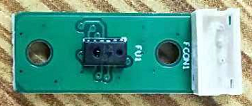
\includegraphics{tof-picture.png}
\caption{Overhead view of the TOF module.}
\end{figure}

\modelno is a high-performance time-of-flight (TOF) module, which can measure
distances optically. This module consists of two chipsets, including a single
photon avalanche diode (SPAD) and an infrared photodiode coupled with an
infrared optical bandpass filter.

This module sensor adopts the TDC electric circuit system, and has good
crosstalk characteristics. The \modelno module performs crosstalk calibration
automatically. The automatically calibrated, highly precise measurement
stability allows for accurate distance measurement even with fingerprints and
smudges. The \modelno module also has strong anti-light interference, and
measures distances independent of object reflectivity, ambient temperature, and
working time.
\section{Product Features}
\begin{itemize}
	\item PSD, infrared LED, and signal processing circuit built-in.
	\item Short measurement cycle (16.5 ms).
	\item Distance measurement range 2.5--10 cm.
	\item Efficient usage of volume (21.0\x7.6\x1mm).
	\item Digital I2C output.
\end{itemize}

\section{Applications}
\begin{itemize}
	\item Robot vacuums.
	\item Industrial robots.
	\item Autonomous vehicles or drones.
	\item User interaction interface.
	\item Any other test or measurement equipment.
\end{itemize}

\section{Figures}
\begin{figure}[H]
\center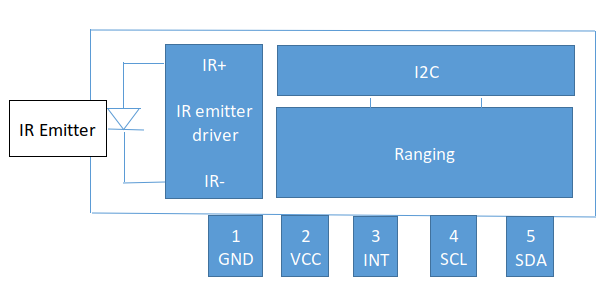
\includegraphics[width=0.9\textwidth]{schematic.png}
\caption{Product diagram of the \modelno module.}
\end{figure}

\begin{figure}[H]
\center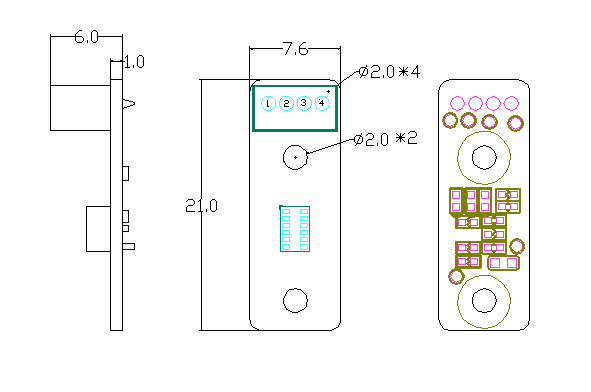
\includegraphics[width=\textwidth]{schematic2.png}
\caption{Dimensions of the \modelno module. Units are in mm.}
\end{figure}

\section{Detailed Specifications}
\ptable{tables/pin_layout.csv}{Interface definition of the \modelno module.}

\begin{figure}[H]
\center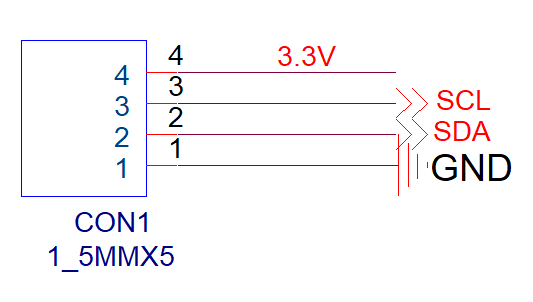
\includegraphics[width=0.5\textwidth]{pins.png}
\caption{Pin layout of the \modelno module.}
\end{figure}

\ptable{tables/operating_ranges_en.csv}{Recommended working ranges of the \modelno module.}

\ptable{tables/maximum_rating_en.csv}{Absolute maximum ranges of the \modelno module.}

\section{Crosstalk Calibration}
Figure \ref{fig:no_cover} demonstrates the distance-response histogram without a
glass cover panel between the TOF sensor and the object, while Figure
\ref{fig:cover} represents the distance-response histogram with a thin glass
cover panel directly in front of the TOF sensor. Without crosstalk calibration,
the TOF sensor inaccurately measures distances even following initial
calibration. However, with the special crosstalk calibration firmware built into
the \modelno module, the \modelno module is able to maintain an accurate, linear
distance-response curve even with a glass panel causing crosstalk feedback, as
shown in Figure \ref{fig:curve}.

\begin{figure}[H]
\center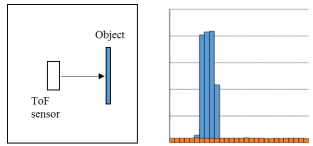
\includegraphics[width=0.8\textwidth]{hist_no_glass.png}
\caption{Histogram without cover glass.}
\label{fig:no_cover}
\end{figure}

\begin{figure}[H]
\center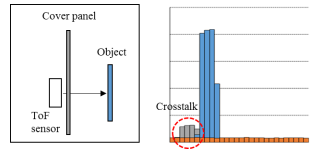
\includegraphics[width=0.8\textwidth]{hist_glass.png}
\caption{Histogram with cover glass.}
\label{fig:cover}
\end{figure}

\begin{figure}[H]
\center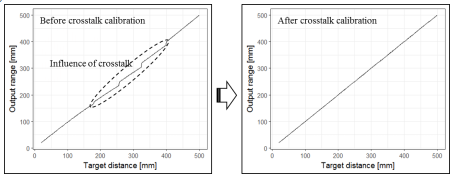
\includegraphics[width=0.9\textwidth]{crosstalk_calib.png}
\caption{Distance response curve before and after crosstalk calibration.}
\label{fig:curve}
\end{figure}

\pchapter{Liability}
FRUITION CO., LTD. does not hold itself liable for any damage caused by improper
use of equipment that does not meet the conditions specified in the relevant
specification sheet, pushing the module past its operating range, or failing to
meet any other specified working conditions.

\end{CJK*}
\end{document}
%%%%%%%%%%%%%%%%%%%%%%%%%%%%%%%%%%%%%%%%%%%%%%%%%%%%%%%%%%%%%%%%%%%%%%%%%%%%%%%%
